\section{Policy Improvement}

\begin{frame} 
\mode<presentation>{
    \begin{center} \huge
        \secname
    \end{center}  
    \begin{center}
    updating the policy to yield a better state value function and state-action value function
    \end{center}
    }
\end{frame}

\subsection{Greedy policy}

\begin{frame}\frametitle{\secname:~\subsecname}

\only<1>{
	The optimal policy is found by:

	\begin{align}
	\pi^* = \argmax_{\pi} V^\pi(\vec x) = \argmax_{\pi} Q^\pi(\vec x, \vec a)\\
	\end{align}

	The above boils down to selecting the best action when at some state $\vec x$:

	\begin{equation}
		\vec a_l = \argmax_{1\leq k \leq A} Q^\pi(\vec x_i, \vec a_k)
	\end{equation}
}
\only<2,3>{
	The greedy\footnote{``greedy'' is to try and get closer to the ``globally'' optimal choice by making ``locally'' optimal decisions} policy method decides on a new policy $\pi'$ using the Q-value function, by:	

	\begin{equation}
	   \pi'(\vec a_k | \vec x_i) = \left\{
	   \begin{array}{ll}
		 1, &\text{if } k = \argmax_{1 \leq l \leq A} Q^\pi(\vec x_i, \vec a_l) \\
		 0, &\text{else.}
	   \end{array}
	   \right.
	\end{equation}
}
\only<3>{
\mode<presentation>{
\begin{center}
		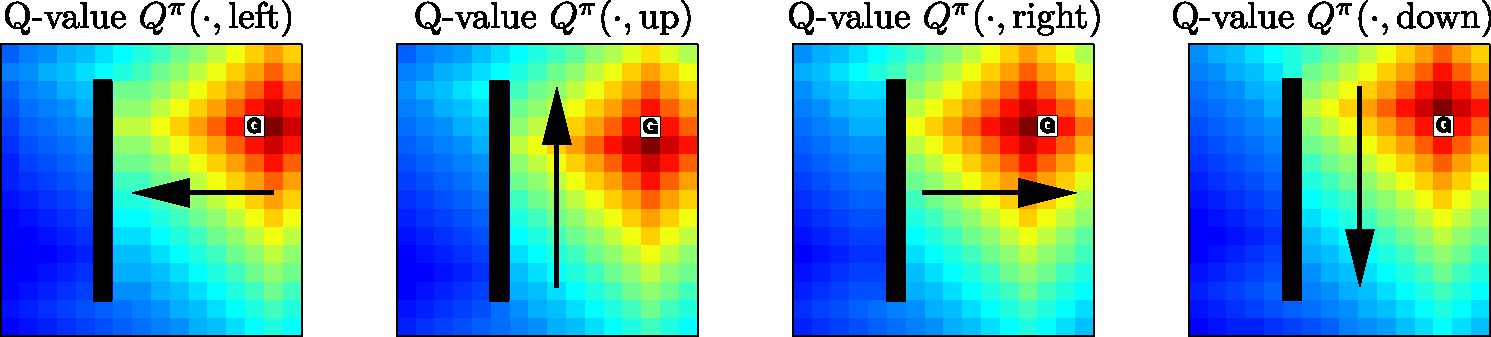
\includegraphics[width=\notesonly{0.9}\textwidth]{img/nav_qvalues}
\end{center} 
}
}

\end{frame}

\subsection{Policy improvement theorem}

% -----------------------------------------------------------------------------
\begin{frame}[label=policy_improvement] \frametitle{\subsecname}
	\begin{itemize}
		\item A policy $\pi'$ is equal or better than a policy $\pi$, i.e.
			\begin{equation*}
				V^{\pi'}(\vec x) \geq V^\pi(\vec x)
			\end{equation*}
			for all states $\vec x$, if:
			\begin{equation*}
				Q^\pi \left(\vec x, \vec a^{\pi'}_{(\vec x)} \right) \geq V^\pi(\vec x)
			\end{equation*}
		\vspace{2mm}		
		\item $Q^\pi \left(\vec x, \vec a^{\pi'}_{(\vec x)} \right)$ is the value of action $\vec a^{\pi'}_{(\vec x)}$ according to policy $\pi'$ at $\vec x$\\[3pt] when following policy $\pi$ afterwards
	\end{itemize}
	
	%\blfootnote{\hfill\hyperlink{policy_improvement_proof}{\beamerbutton{derivation here}}}
\end{frame}

\subsection{Policy iteration}

% -----------------------------------------------------------------------------
\begin{frame} \frametitle{\subsecname}
		\vspace{1mm}
		\small
		\mbox{
		\hspace{-4mm}
		Any policy $\pi_i$ is {\em improved} by
			the greedy policy $\pi_{i+1}$ operating on $\pi_i$'s Q-values $Q^{\pi_i}$:}
			\vspace{1mm}	
			\begin{align*}
				V^\pi(\vec x_i) &= \sum_{k=1}^{A} \pi(\vec a_k | \vec x_i) \; Q^\pi(\vec x_i, \vec a_k) \\
				&\leq \max_k Q^\pi(\vec x_i, \vec a_k) \overset{!}{=} Q^\pi \left(\vec x, \vec a^{\pi'}_{(\vec x)} \right)
			\end{align*}
		%\vspace{4mm}
		%\item alternating value estimation and policy improvement 
		\normalsize
	\vspace{4mm}
	\begin{block}{Policy iteration (PI)}
		initialize policy $\pi_{0}$ randomly\\
		\While{Q-values not converged}{
			estimate 
				%(with any algorithm) Q-value function 
				$\tilde Q^{\pi_i} :\approx Q^{\pi_i}$ of policy $\pi_i$ (estimation of Q-values via e.g. SARSA for $\pi_i$)\\
			choose $\pi_{i+1}$ to be the greedy policy on $\tilde Q^{\pi_i}$
		} 
		
		\vspace{-4mm}
		{\footnotesize\hfill\citep[see]%
		[for convergence with estimated Q-values]{Bertsekas07}}
	\end{block}	
\end{frame}

\subsection{On-line off-policy improvement: Q-learning}

\begin{frame}\frametitle{\subsecname}

Q-learning is an on-line off-policy improvement method, which integrates greedy policy improvement into off-policy TD learning.

\begin{block}{Q-learning}
	Pick a sampling policy $\pi$. (It will typically depend on the current Q-values.)
	\slidesonly{\vspace{-3mm}}
	\begin{align}
			\tilde Q_{(t+1)}^*(\vec x^{(t)}, \vec a^{(t)})
			\;\;=\;\;&
			\tilde Q_{(t)}^*(\vec x^{(t)}, \vec a^{(t)})
			\\
			&\kern-10ex
			 \;+\; \lr \Big( \underbrace{
				{\color{reward}r^{(t)}} + \gamma 
				\overbrace{
					{\color{policy} \max_{1 \leq k\leq A}}
					\tilde Q_{(t)}^*({\color{trans}\vec x^{(t+1)}}, 
						{\color{policy}\vec a_k})
				}^{\text{\scriptsize \kern-2exgreedy policy improvement\kern-2ex}}
				- \, \tilde Q_{(t)}^*(\vec x^{(t)}, \vec a^{(t)})	
				}_{\text{\scriptsize TD-error} \displaystyle \scriptstyle \;\Delta Q_{(t)} }\Big)
	\end{align}
\end{block}
	
	\only<1>{
	$\Delta Q_{(t)}$ in SARSA for comparison:
	\begin{equation}
			\Delta Q_{(t)} = {\color{reward} r^{(t)}} \, + \, \gamma \, \tilde{Q}^\pi_{(t)} ({\color{trans}  \vec x^{(t+1)}},\,{\color{policy}  \vec a^{(t+1)}} ) - \tilde{Q}^\pi_{(t)} ( \vec x^{(t)},\, \vec a^{(t)} )
	\end{equation}
	}
	\only<2>{
	
	\slidesonly{\vspace{-3mm}}
	
	\question{How do we extract the optimal policy $\pi^*$?}\\
	
	\slidesonly{\vspace{-5mm}}
	
	\notesonly{
	 - Extracting the optimal policy is done the same way as by the greedy policy:
	 }
	\begin{equation}
	   \pi^*(\vec a_k | \vec x_i) = \left\{
	   \begin{array}{ll}
		 1, &\text{if } k = \argmax_{1 \leq l \leq A} Q^*(\vec x_i, \vec a_l) \\
		 0, &\text{otherwise.}
	   \end{array}
	   \right.
	\end{equation}
	}

\end{frame}

\begin{frame}\frametitle{\subsecname}

Q-learning \citep{Watkins92}:
\begin{itemize}
\item online policy improvement
\item estimates the Q-value function of an optimal (unknown) policy $\pi^*$
\item off-policy with sampling policy $\pi$
\item effectively TD learning with greedy policy imporvement
\item Q-learning is a contraction mapping for \emph{any} ergodic Markov chain
			\begin{equation}
				\lim\limits_{p \to \infty} \E \Big\lbrack
					\smallsum{t=0}{p} \Delta Q_t \Big\rbrack
				= Q^{\pi^*}
			\end{equation}
\item Q-learning is the only on-line off-policy algorithm for policy improvement.
\end{itemize}

\end{frame}
